\documentclass[11pt]{beamer}
\usepackage[utf8]{inputenc}
\usepackage[german]{babel}
\usepackage[T1]{fontenc}
%\usepackage[usefilenames, RMstyle=Light, SSstyle=Light, TTstyle=Light, DefaultFeatures={Ligatures=Common}]{plex-otf} 
\usepackage{amsmath}
\usepackage{amsfonts}
\usepackage{amssymb}
\usepackage{graphicx}
\usepackage{multirow}
\usepackage{array}
\newcolumntype{M}[1]{>{\centering\arraybackslash}m{#1}}
\usetheme{Dresden}
\author{Felix Beckmann, Leonhard Alkewitz, Max Lautenbach}
\title{Die Optimierung der Energiebilanz von simulierten Gebäuden mithilfe eines evolutionären Algorithmus}
%\setbeamercovered{transparent} 
%\setbeamertemplate{navigation symbols}{} 
\logo{
\includegraphics[scale=.05]{logo.png}} 
\institute{Spezialschulteil des Albert-Schweizer Gymnasium Erfurt} 
\date{\today} 
%\subject{} 
\begin{document}

\begin{frame}

\end{frame}

\begin{frame}
\begin{center}
\huge{2 376 000 000 000 000 $J$}  \\  
\pause \huge{641 000 000 $kWh$} \\ 
\pause \huge{81 000 000 $kg$ $SKE$ \footnote{SKE = Steinkohleeinheit}} \\ 
\hrulefill{}  \\
\pause \huge{2000-2500 $l$} \\ 
\pause \huge{10-15 $Badewannen$}
\end{center}
\end{frame}

\begin{frame}
\titlepage
\end{frame}

\begin{frame}{Gliederung}
\begin{enumerate}
\item{Einführung in die Thematik der Optimierung und der Energiebilanz von Gebäuden}
\begin{enumerate}
\item{Verfahren zur evolutionären Optimierung}
\item{Ermittlung der Energiebilanz von Gebäuden}
\end{enumerate}
\item{Zielstellung der Seminarfacharbeit und Abgrenzung des Themas}
\item{Methodik zum Erreichen unserer Ziele}
\item{Motivation und Begründung zur Wahl dieses Themas}
\end{enumerate}
\end{frame}

\begin{frame}{Einführung in die Thematik der Optimierung und der Energiebilanz von Gebäuden}
\framesubtitle{\large{\textcolor{black}{Verfahren zur evolutionären Optimierung:}}}
\begin{figure}
\includegraphics[scale=0.12]{Scan9}
\caption{Optimierung nach dem Vorbild der Evolution}
\end{figure}
\end{frame}

\begin{frame}{Einführung in die Thematik der Optimierung und der Energiebilanz von Gebäuden}
\framesubtitle{\large{\textcolor{black}{Ermittlung der Energiebilanz von Gebäuden:}}}
\begin{figure}
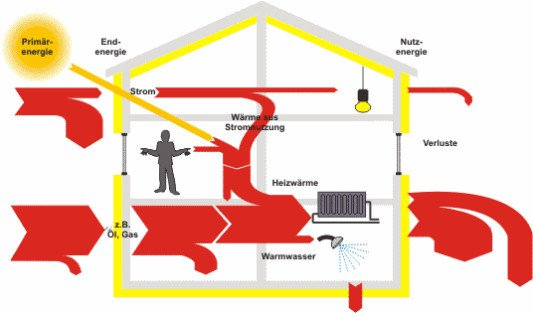
\includegraphics[scale=0.45]{0dd5dc31023435ef-2.jpg} 
\caption{Energiebilanz eines Wohngebäudes}
\end{figure}
\end{frame}

\begin{frame}{Zielstellung der Seminarfacharbeit und Abgrenzung des Themas}
\begin{itemize}
\item{Aneignen von themenbezogenem Fachwissen}\pause
\item{Erstellung einer Simulation unter Berücksichtigung von Bedingungen}\pause
\item{Anwendung von EA\footnote{EA = evolutionärer Algorithmus}}\pause
\item{graphische Ausgabe der evolvierten Gebäude}\pause
\item{Abgrenzung des Themas}\pause
\begin{itemize}
\item{Spezialisierung auf Wohngebäude}
\item{Begrenzung auf Grundlagen der Statik und Werkstoffkunde}
\item{detaillose Darstellung der Gebäude}
\item{keine zusätzliche Energiequelle, z.B. Solartechnik} 
\end{itemize}
\end{itemize}
\end{frame}

\begin{frame}{Methodik zum Erreichen unserer Ziele}
\begin{footnotesize}
\begin{tabular}{|M{2cm}||M{2.5cm}|M{2.5cm}|M{2.5cm}|} \hline
   Datum & Leonhard & Felix & Max \\ \hline \hline
   \multirow{2}*{Oktober 2018} & \multicolumn{3}{|M{7.5cm}|}{Literaturrecherche und Javakenntnisse auffrischen} \\ \cline{2-4}
   & Bauphysik & 3D Graphik & evolutionäre \newline Algorithmen \\ \hline
   November 2018 & Wissenstand über Architektur erweitern  & \multicolumn{2}{|M{5cm}|}{Ansätze der Simulation: Objekt \textit{Haus} mit grundlegenden Eigenschaften}\\ \hline
   Dezember 2018 & Statikkenntnisse aneignen & Sachverstand über 3D Graphik erweitern & Rahmen für EA: \newline Einbinden in Simulation\\ \hline
   Januar 2019 & Physik des Energieverlustes & Modellierung von Hausmodulen\footnote{Haus wird aus mehreren Modulen aufgebaut} & Methoden der Vererbung von EA implementieren \\ \hline   
   Februar 2019 & \multicolumn{3}{|M{7.5cm}|}{Puffer} \\ \hline
\end{tabular}
\end{footnotesize}
\end{frame}

\begin{frame}{Methodik zum Erreichen unserer Ziele}
\begin{footnotesize}
\begin{tabular}{|M{2cm}||M{2.5cm}|M{2.5cm}|M{2.5cm}|} \hline
   Datum & Leonhard & Felix & Max \\ \hline \hline
   März 2019 & wichtige Werte für Energiebilanz in Programm einbinden & Grundlage für Module in Programm einbinden & Verfassen Kapitel zu Optimierung \\ \hline
   April 2019 & Energiequellen herausarbeiten & \multicolumn{2}{|M{5cm}|}{Wissen über Architektur in Programm einbinden} \\ \hline
   Mai 2019 & Verfassen Kapitel zu Statik und Architektur & \multicolumn{2}{|M{5cm}|}{Sachverständnis zu thermalen Austausch von Haus in Simulation einbinden} \\ \hline
   Juni 2019 & Verfassen der Kapitel zu thermalen Austausch & graphische Implementierung von Modulen & Methode zu Energiebilanzberechnung \\ \hline
   Juli 2019 & \multicolumn{3}{|M{7.5cm}|}{Puffer} \\ \hline
   August 2019 & Beispieldurchlauf und Ergebnisdokumentation & Verfassen der Kapitel zu 3D Graphik & Beispieldurchlauf und Ergebnisdokumentation \\ \hline
\end{tabular}
\end{footnotesize}
\end{frame}

\begin{frame}{Methodik zum Erreichen unserer Ziele}
\begin{footnotesize}
\begin{tabular}{|M{2cm}||M{2.5cm}|M{2.5cm}|M{2.5cm}|} \hline
   Datum & Leonhard & Felix & Max \\ \hline \hline
   September 2019 & Fehleranalyse und -berichtigung & Visualisierung der Ergebnisse & Fehleranalyse und -berichtigung \\ \hline
   Oktober 2019 & Verfassen der Kapitel zu Simulation & Visualisierung der Ergebnisse & Verfassen der Kapitel zu Simulation \\ \hline
   November 2019 & Verfassen der Kapitel zu Simulation & Ausbesserung von graphischen Fehlern & Ausbessern von programmierten Fehlern \\ \hline
   Dezember 2019 & \multicolumn{3}{|M{7.5cm}|}{Korrekturlesen und Abgabe der Seminarfacharbeit} \\ \hline
    Januar 2020 & \multicolumn{3}{|M{7.5cm}|}{Sicherstellung der Lauffähigkeit des Programms und graphische Vorbereitung auf Verteidigung} \\ \hline
     Februar 2020 & \multicolumn{3}{|M{7.5cm}|}{Erstellung der Präsentation und Beispielen} \\ \hline
      März 2020 & \multicolumn{3}{|M{7.5cm}|}{Vorbereitung des Kolloquiums} \\ \hline
\end{tabular}
\end{footnotesize}
\end{frame}
\begin{frame}{Motivation und Begründung zur Wahl dieses Themas}
\begin{itemize}
\pause
\item{hohes Potential der Verbesserung der Energiebilanz von Wohngebäuden}\pause
\item{Affinität zur Informatik, Architektur und Bauphysik}\pause
\item{Verbinden von Informatik und Physik mittels Anwendung EA auf Bauphysik}\pause
\item{automatisierte Planung von Häusern unter Einbezug von Energiebilanz und Statik}\pause
\item{Entdecken möglicher unkonventioneller, unbekannter Hausformen}
\end{itemize}
\end{frame}

\begin{frame}
\begin{figure}
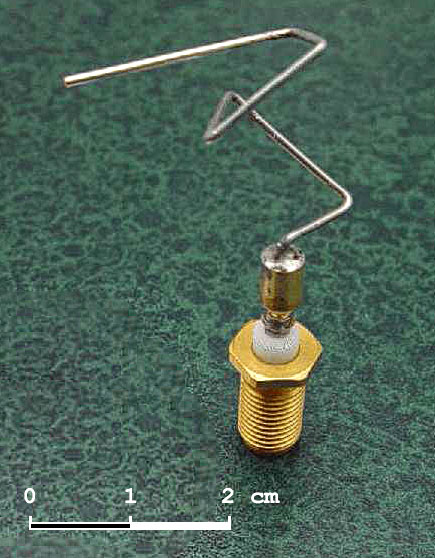
\includegraphics[scale=0.34]{St_5-xband-antenna.jpg} 
\caption{Eine von EA optimierte Antenne}
\end{figure}
\end{frame}

\begin{frame}{Literaturquellen}
\begin{thebibliography}{9}
\bibitem{1}
\textcolor{black}{
Graf, Anton; Neue Passivhäuser; Verlag Georg D.W. Callwey, München, 2003}
\bibitem{2}
\textcolor{black}{\url{https://www.bmwi.de/Redaktion/DE/Downloads/Energiedaten/energiedaten-gesamt-pdf-grafiken.pdf?__blob=publicationFile&v=38}; zuletzt besucht: 26.09.2018}
\bibitem{3}
\textcolor{black}{
\url{https://ag-energiebilanzen.de/index.php?article_id=29&fileName=ausw_30jul2018_ov.pdf}; zuletzt besucht: 26.09.2018}
\end{thebibliography}
\end{frame}

\begin{frame}{Bildquellen}
\begin{thebibliography}{9}
\bibitem{4}
\textcolor{black}{
\textit{Abbildung 1}; Prof. Dr. Markl, Jürgen; Markl Biologie; S. 256.1; 1. Auflage; Ernst Klett Verlag, Stuttgart, 2010}
\bibitem{5}
\textcolor{black}{
\textit{Abbildung 2}; \url{https://www.baunetzwissen.de/imgs/5/7/5/8/5/3/0dd5dc31023435ef.jpg}; zuletzt besucht: 27.09.2018}
\bibitem{6}
\textcolor{black}{
\textit{Abbildung 3}; \url{https://upload.wikimedia.org/wikipedia/commons/f/ff/St_5-xband-antenna.jpg}; zuletzt besucht: 27.09.2018}
\end{thebibliography}
\end{frame}
\end{document}
